% Modelo de slides para projetos de disciplinas do Abel
\documentclass[10pt]{beamer}

\usetheme[progressbar=frametitle]{metropolis}
\usepackage{appendixnumberbeamer}
\usepackage[numbers,sort&compress]{natbib}
\bibliographystyle{plainnat}

\usepackage{booktabs}
\usepackage[scale=2]{ccicons}

\usepackage{xspace}
\newcommand{\themename}{\textbf{\textsc{metropolis}}\xspace}

\title{Physik GFS - Erdmagnetfeld}
% \subtitle{Subtítulo}
% \date{\today}
\date{23.01.2020}
\author{Valentin Zwerschke}
\institute{Königin Olga Stift - Stuttgart}
% \titlegraphic{\hfill\includegraphics[height=1.5cm]{logo.pdf}}

\begin{document}

\maketitle

\begin{frame}{Gliederung}
  \setbeamertemplate{section in toc}[sections numbered]
  \tableofcontents[hideallsubsections]
\end{frame}
\section{Was ist das Erdmagnetfeld und wie wird es genutzt?}
\begin{frame}{Was ist das Erdmagnetfeld und wie wird es genutzt?}
        \begin{minipage}[c]{7cm}
            \textbf{Was ist das Erdmagnetfeld?}\pause
            \begin{itemize}
                \item Das Erdmagnetfeld kann man wie das Feld eines großen Stabmagneten beschreiben \pause
                \begin{itemize}
                   % \item Magnetischer Nordpol ungefähr beim geographischen Südpol
                    \item Magnetischer Südpol liegt ungefähr beim geographischen Nordpol\pause
                    \item "Magnetische" Achse und Rotationsachse sind um ca. 11° geneigt\pause
                \end{itemize}
                \item Ein Magnetfeld wird mitttels Feldlinen beschieben\pause
                
                \begin{itemize}
                \item Diese verlaufen vom Nord- zum Südpol\pause
                    \item Magnetfeld zeigt entlang der Linien in Richtung Südpol \pause
                    \item Dichte der Linien zeigt Magnetfeldstärke an\pause
                \end{itemize}
            \end{itemize}
    \end{minipage}
    \begin{minipage}[c]{3cm}
    \hspace{1cm}
        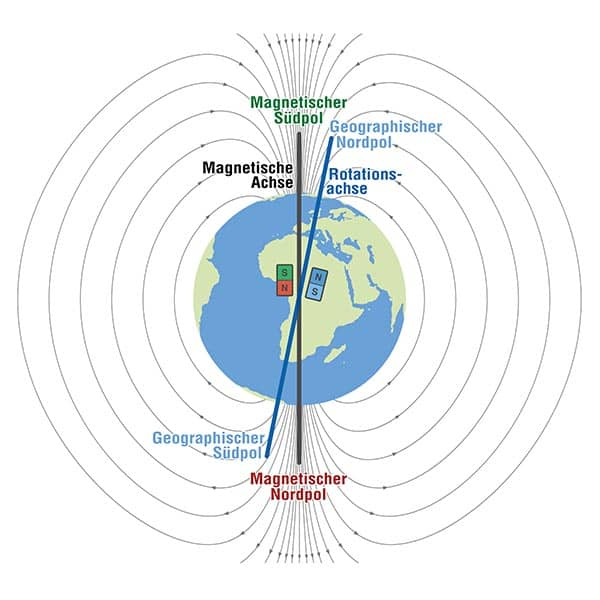
\includegraphics[height = 5cm]{Erdmagnetfeld-und-Rotation.jpg}
    \end{minipage}
\end{frame}

\begin{frame}{Was ist das Erdmagnetfeld und wie wird es genutzt?}
    \begin{minipage}[c]{0.7\textwidth}
    \vspace{1cm}
    \textbf{Deklination (auch Missweisung):}\pause
        \begin{itemize}
            \item Winkel zwischen der Magnetfeldrichtung (wo die Kompassnadel hinzeigt)
             und der geographischen Nordrichtung
            \item Bei Nutzung eines Kompasses zu beachten!\pause
            \vspace{0.5cm}
    \end{itemize}
\end{minipage}
\begin{minipage}[c]{0.25\textwidth}
    %\hspace{5cm}
    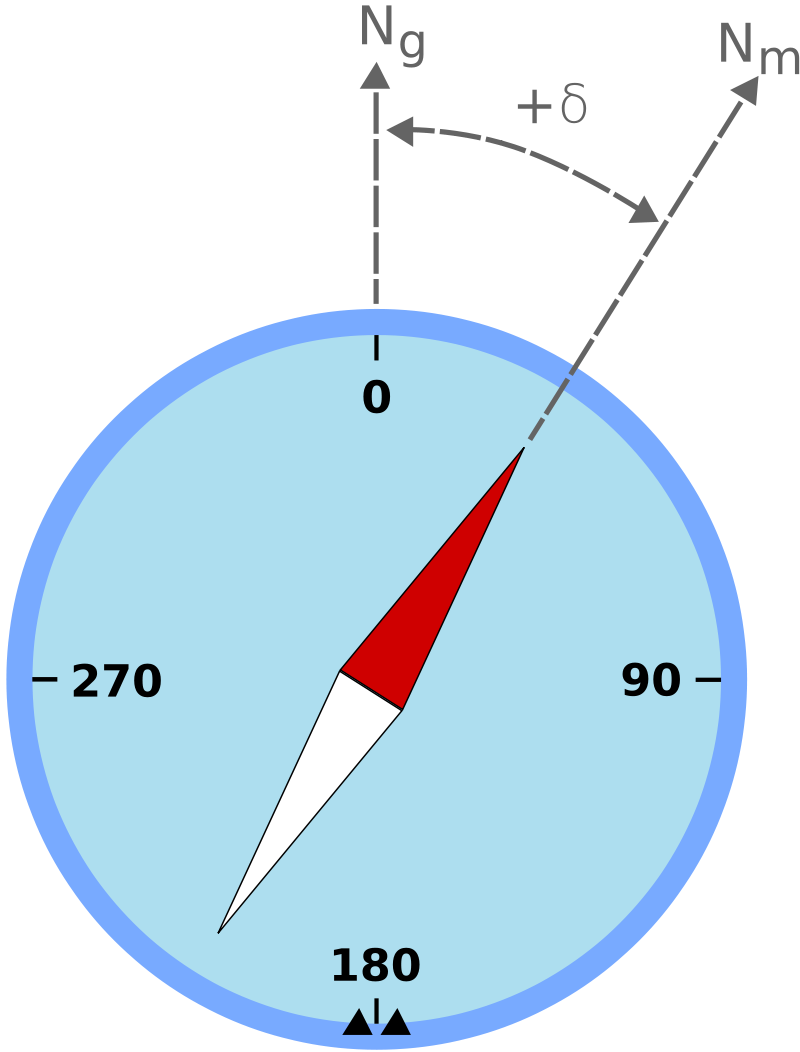
\includegraphics[height = 3cm]{Deklination.png}
\end{minipage}

\begin{minipage}[b]{0.7\textwidth}
\textbf{Inklination:}\pause
    \begin{itemize}
        \item Neigung der Feldlinien des Erdmagnetfeldes gegen die Horizontale\pause
    \end{itemize}
\end{minipage}
\begin{minipage}[c]{0.25\textwidth}
    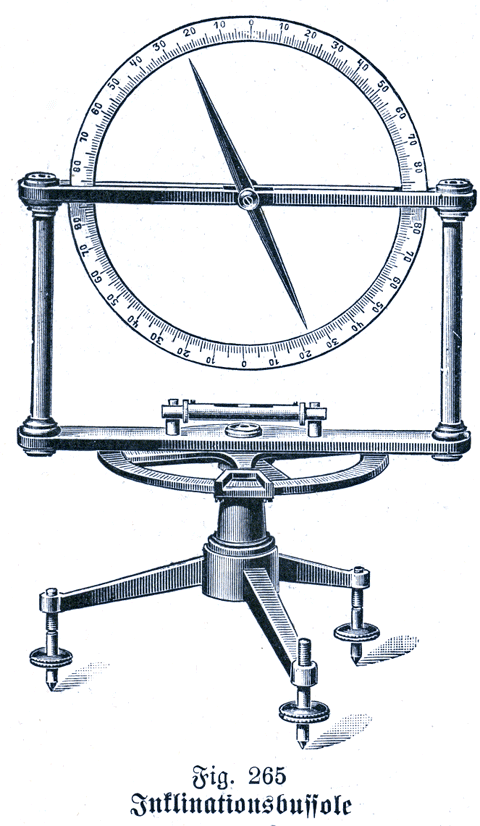
\includegraphics[height = 3.5cm]{Inklinationsbussole.png}
\end{minipage}
\end{frame}

\begin{frame}{Was ist das Erdmagnetfeld und wie wird es genutzt?}

\textbf{Das Erdmagnetfeld besteht eigentlich aus drei Komponenten:}\pause
\begin{enumerate}
   \item Hauptteil des Magnetfelds (ca. 95\%) durch Ströme \textbf{im flüssigen, äußeren Erdkern} erzeugt (Geodynamo)\pause
    \item  Kleinerer Teil (ca. 1 bis 3 \%) durch elektrische Ströme \textbf{in der Ionosphäre} (hoch gelegene Schicht in der Erdatmosphäre, in der viele geladene Teilchen sind) und \textbf{in der Magnetosphäre} \pause
    \item Ein weiterer kleiner Teil (bis zu mehrerern \%), der räumlich stark variiert und durch remanente Magnetisierung von Stoffen \textbf{in Teilen der oberen Erdkruste} hervorgerufen wird, z.B. bei Erzlagerstätten.\pause
\end{enumerate}
\end{frame}

\begin{frame}{Was ist das Erdmagnetfeld und wie wird es genutzt?}
\textbf{Warum ist das Erdmagnetfeld so immens wichtig für Mensch \& Tier?}\pause
\begin{itemize}
    \item Es schützt das Leben auf der Erde! \pause
    \item Viele Tiere nutzen es zur Orientierung, einige Beispiele:\pause
    \begin{itemize}
        \item \textbf{Lachse} orientieren sich über Feldstärke und Inklination auf dem Weg zurück zum Geburtsort (angeborene Magnetische Landkarte)\pause
        \item \textbf{Tauben} sind Meister der Langstreckennavigation und verfügen über exzellente Fähigkeiten, das Magnetfeld der Erde wahrzunehmen (Rezeptorten vermutlich im Innenohr) \pause
        \item \textbf{Zugvögel} können vermutlich die Himmelsrichtung bestimmen als auch ihre geografische Breite\pause
        \item Weitere Tiere: Termiten, Ameisen, Hunde, Wale, ...\pause
    \end{itemize}
    \item Auch Menschen nutzen es zur Navigation, z.B. mit Kompass
\end{itemize}
    
\end{frame}
%\begin{frame}{Zugvögel und wie sie sich orientieren}
%\textbf{Wie orientieren sich die Zugvögel}
 %   \begin{itemize}
 %       \item Zugvögel orientieren sich Teilweise an den Feldlinien vom %Erdmagnetfeld
 %   \end{itemize}
%\end{frame}
\section{Erste Entdeckung des Erdmagnetfelds}
\begin{frame}{Erste Entdeckung des Erdmagnetfelds}
    \textbf{Frühe Entdeckungsgeschichte des Erdmagnetismus}\pause
    \begin{itemize}
    \item Chinesen und Mongolen erkannten die Nordweisung magnetisierter Körper schon \textbf{vor mehr als tausend Jahren}. \pause
    %\item Chinesen strichen mit bestimmten Steinen über eine Eisennadel.
    %\item sie hängten sie dann frei beweglich aus -> Nadel richtet sich in Nord-Süd Richtung aus.
    \item Ältester Bericht über die Nutzung eines Kompasses in Europa stammt aus dem Jahr 1190 n. Chr.\pause
    \item Anfang des 14. Jahrhunderts wurde diese „Wundernadel“ zu einer der wichtigsten Grundlagen für Seefahrer wie Columbus\pause
    \item Europäer glaubten zuerst an einen "Magnetberg" im Norden.\pause
    \item Ca. 1600 erkannte \textbf{William Gilbert}, dass die Ursache der Ausrichtung der Kompassnadel die Erde selbst ist.\pause
    \item Messungen durch \textbf{Henry Gellibrand} ergaben, dass das Magnetfeld nicht statisch ist, sondern sich langsam ändert.\pause
    \end{itemize}
\end{frame}

\begin{frame}{Erste Entdeckung des Erdmagnetfelds}
    \textbf{Wissenschaftliche Erforschung des Erdmagnetismus im 19. Jh.}\pause
  \begin{itemize}
    \item 1831 entdeckte Michael Faraday die elektromagnetische Induktion und damit die Natur des Magnetismus: Wo elektrischer Strom fließt, entsteht ein Magnetfeld.\pause
    \item Seitdem intensive Forschung und Vermessung des Erdmagnetfeldes\pause
    \item Alexander von Humboldt: Messungen im preußischen Bergbau und auf Forschungsreisen\pause
    \item Carl-Friedrich Gauß: gründet erstes geophysikalisches Observatorium.\pause
    % \item Der gegründete Magnetische Verein lieferte Daten
    
    \item Gauß zeigte 1839, dass der Hauptteil des statischen Erdmagnetfeldes aus dem Erdinneren stammt, kleinere, kurzzeitige Variationen dagegen von außerhalb. \pause
\end{itemize}
\end{frame}

\section{Entstehung des Erdmagnetfelds (Dynamotheorie)}
\begin{frame}{Entstehung des Erdmagnetfelds (Dynamotheorie)}
    \textbf{Zur Entstehung des Hauptmagnetfeldes gibt es verschiedene Theorien, Dynamotheorie heute allgemein anerkannt}\pause
  \begin{itemize}
    \item  Erdinnere besteht aus festem, heißem Kern (5000°C) und darüber liegender flüssiger Schicht (im wesentlichen Eisen)\pause 
    \item In der flüssigen Schicht viel Bewegung: Konvektionsströmungen (von heiß nach kalt), die zudem abgelent werden (Corioliskraft) \pause
    \item Resultierende Schraubenförmige Bewegung leitender Materie führt zu Magnetfeld\pause
    \item Sich selbst verstärkender Effekt wie beim Fahrrad-Dynamo --> Daher der Name\pause
\end{itemize}
Leider: kein anschauliches Modell zur Dynamotheorie, an dem der Strom- und Feldlinienverlauf bei den Bewegungen der leitfähigen Flüssigkeit nachvollzogen werden könnte
\end{frame}
\begin{frame}{Entstehung des Erdmagnetfelds (Dynamotheorie)}
\begin{center}
    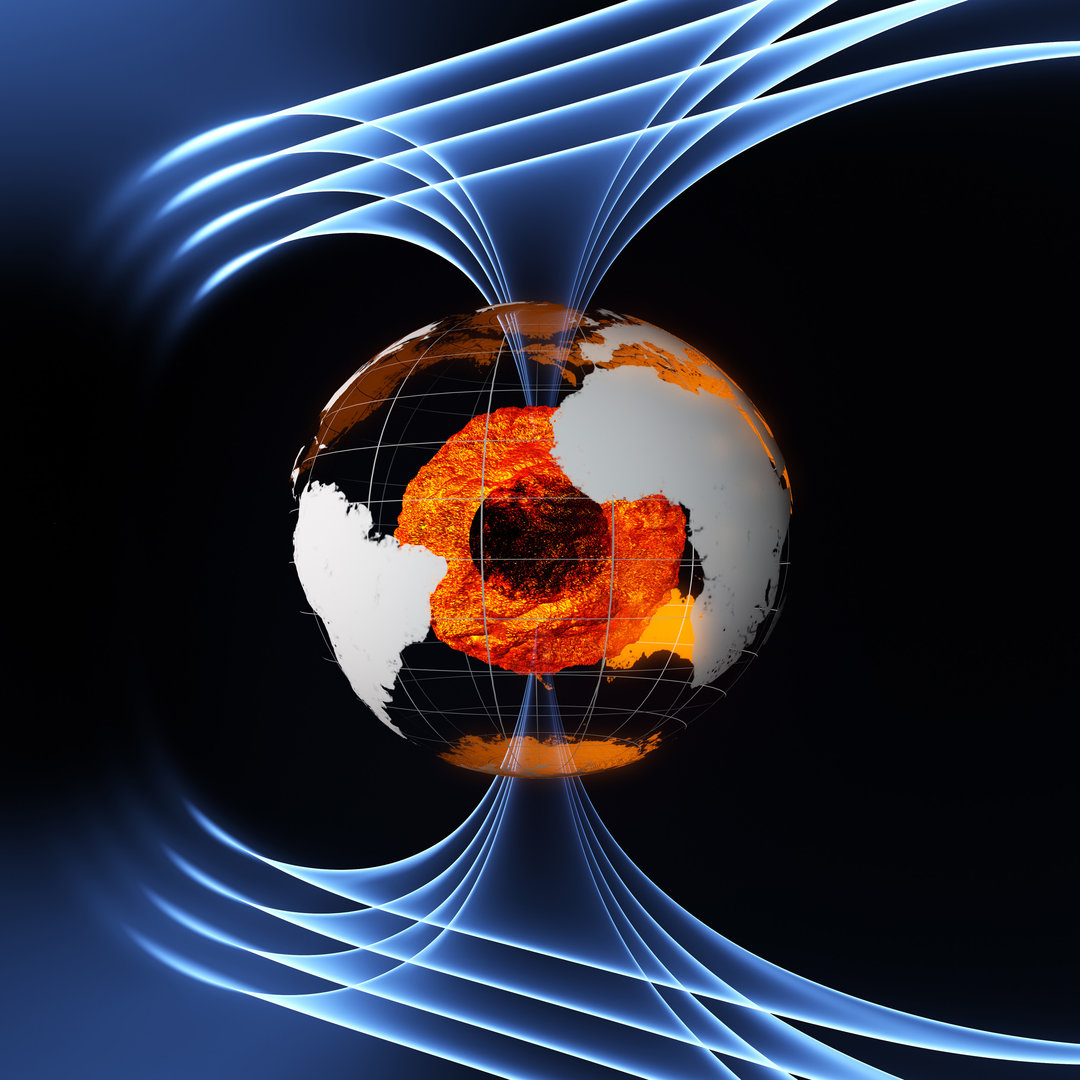
\includegraphics[width=0.7\textwidth]{Earth_s_stormy_heart_pillars.jpg}
\end{center}
\end{frame}


\section{Ist das Magnetfeld statisch und wird es stabil bleiben?}
\begin{frame}{Ist das Magnetfeld statisch und wird es stabil bleiben?}
\textbf{Das Erdmagnetfeld (Hauptfeld) ändert sich stetig}\pause
\begin{itemize}
    \item Die Lage der magnetischen Pole wandert über die Jahre
    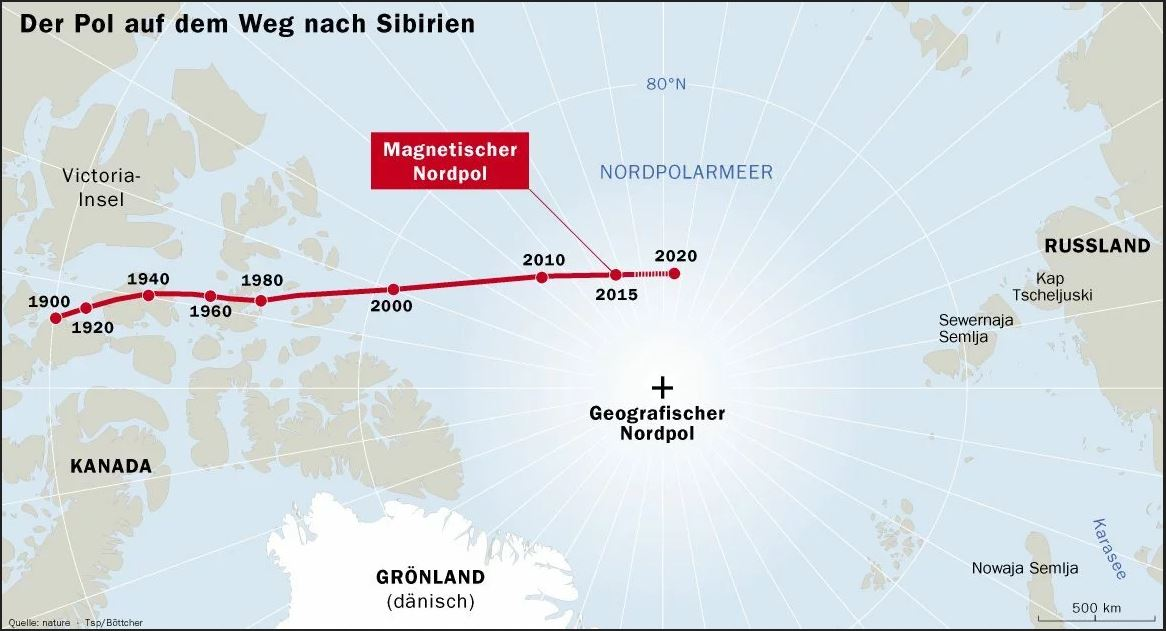
\includegraphics[width=0.6\textwidth]{Polwanderung.jpg}
    \item Feldstärke ändert sich über die Zeit: innerhalb der vergangenen 170 Jahre hat es sich um zehn Prozent abgeschwächt
    
    
\end{itemize}
 %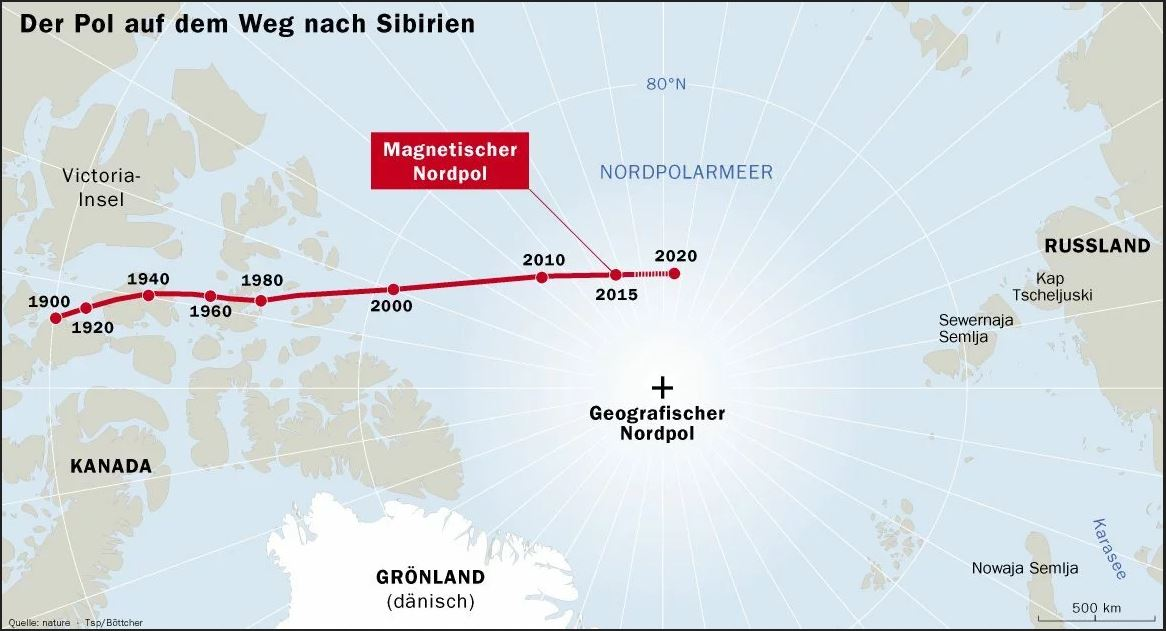
\includegraphics[width=0.6\textwidth]{Polwanderung.jpg}
 %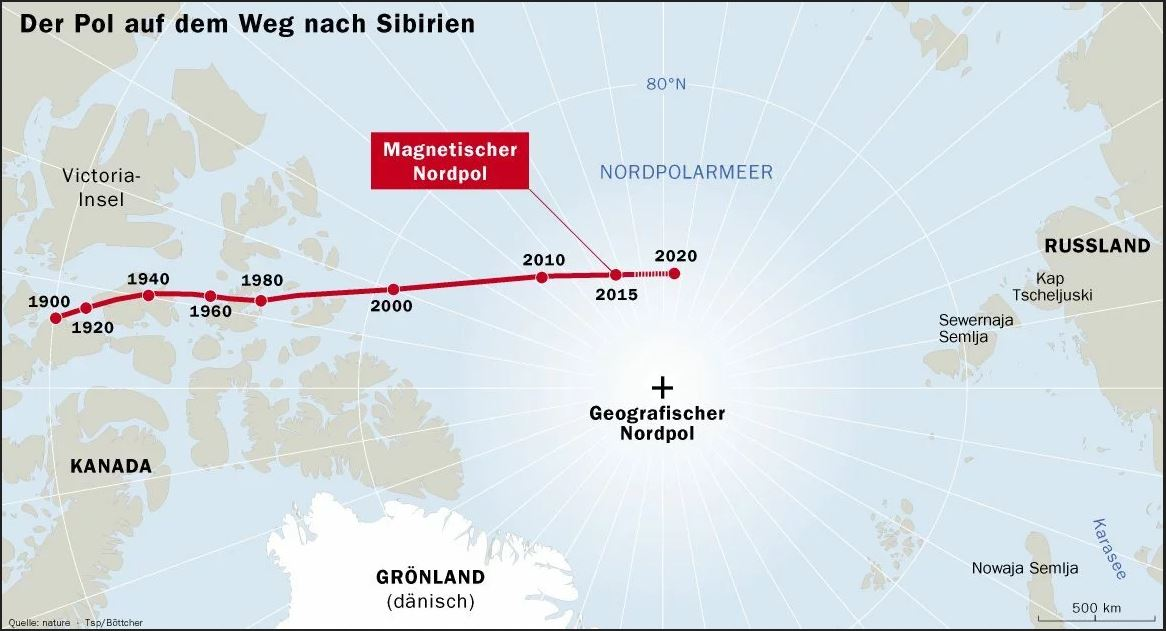
\includegraphics[width=0.3\textwidth]{Polwanderung.webp}
\end{frame}

\begin{frame}{Ist das Magnetfeld statisch und wird es stabil bleiben?}
\textbf{Das Erdmagnetfeld polt sich sogar um}\pause
\begin{itemize}
      
       \item In der Erdgeschichte hat es sich sogar mehrfach umgekehrt \pause
    \item Statisstisch ca. alle 250.000 Jahre\pause
    \item Dabei trudelt das Feld durch Chaos und bricht zeitweise in sich zusammen\pause
    \item Computerberechnungen stützen diese Theorie
      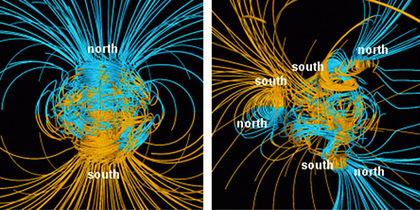
\includegraphics[width=0.6\textwidth]{Erdmagnetfeld-Umpolung}
    
\end{itemize}
 %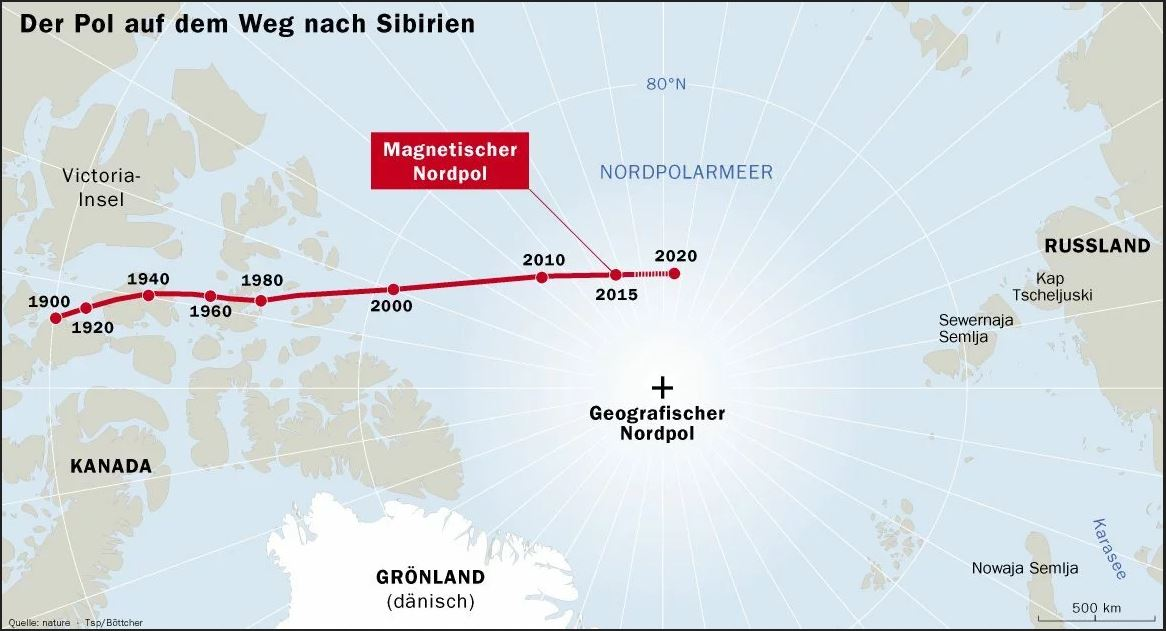
\includegraphics[width=0.6\textwidth]{Polwanderung.jpg}
 %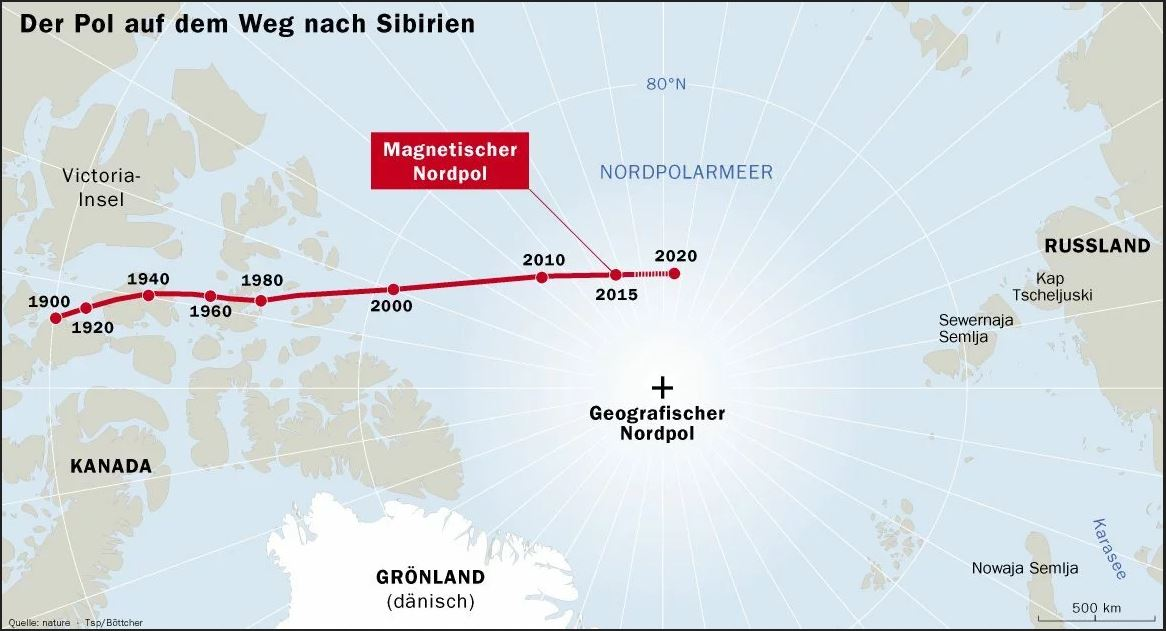
\includegraphics[width=0.3\textwidth]{Polwanderung.webp}
\end{frame}
\section{Inwiefern schützt das Magnetfeld die Erde?}
\begin{frame}{Inwiefern schützt das Magnetfeld die Erde?}
\textbf{Das Erdmagnetfeld ist ein Schild, der vor dem zerstörerischen Strom geladener und energiereicher Partikel – Protonen, Alphateilchen und Elektronen –, die die Sonne auf uns einprasseln lässt, schützt.}
%\begin{itemize}
%    \item ...
%    
%\end{itemize}
\begin{center}
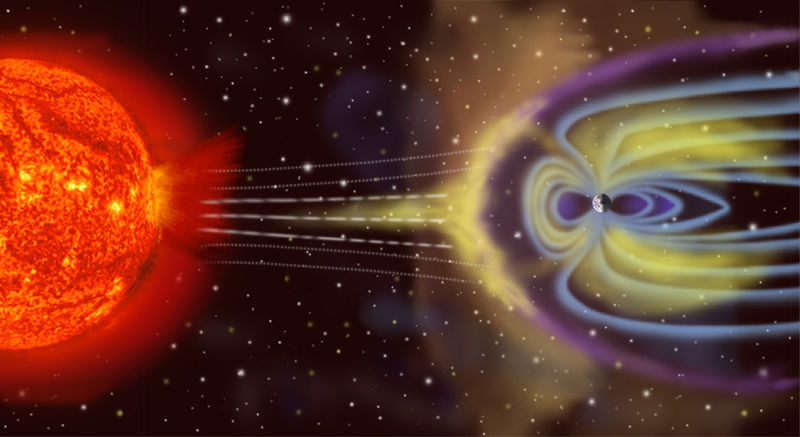
\includegraphics[width=0.9\textwidth]{Sonnenwind.jpg}
\end{center}
\end{frame}

\begin{frame}{Inwiefern schützt das Magnetfeld die Erde?}
\textbf{Das Erdmagnetfeld bringt uns auch die wunderschönen Polarlicher}
\begin{center}
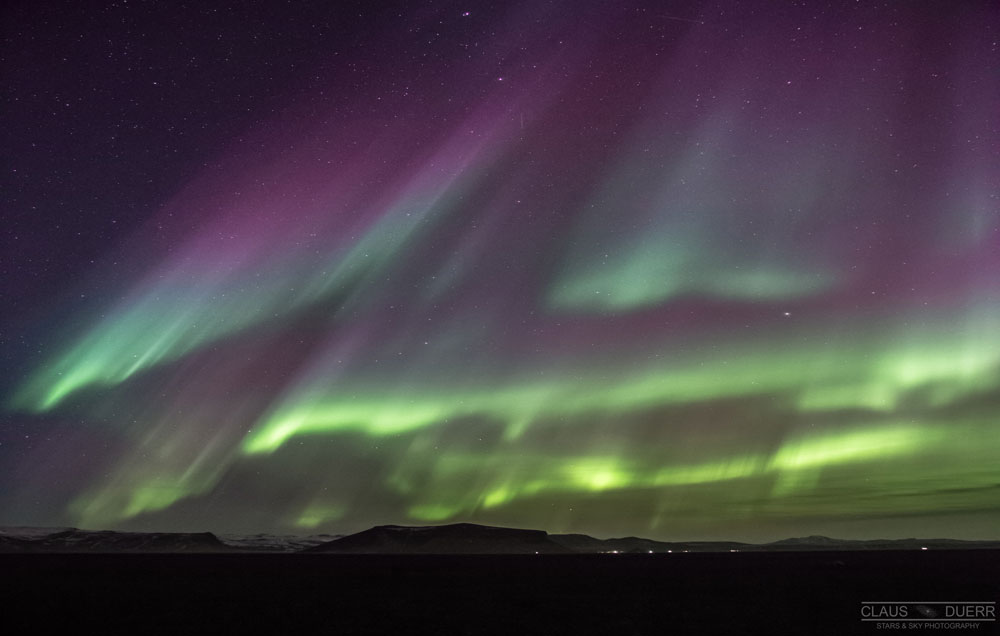
\includegraphics[width=0.9\textwidth]{Bild-6-Starkes-Polarlicht-mit-den-seltenen-blauen-und-lila-Anteilen.jpg}
\end{center}
\end{frame}

\begin{frame}{Inwiefern schützt das Magnetfeld die Erde?}
\textbf{Entstehung eines Polarlichts - Von der Sonne zur Erde}\pause
\begin{itemize}
    \item Sonnenwinde aus Plasma (hauptsächlich Ionen \& Elektronen) erreichen die Erde. \pause
    \item Sie treffen auf das Magnetfeld und drücken es zusammen, ohne jedoch die Atmosphäre erreichen zu können.\pause
    \begin{center}
        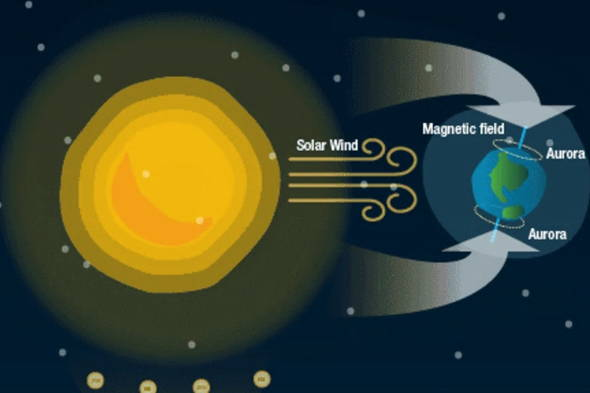
\includegraphics[width=0.4\textwidth]{nordlichter004-590.jpg}\pause
    \end{center}
\item Die geladenen Teilchen fliegen entlang der Magnetfeldlinen um die Erde herum zu den Polarkreisen 
\end{itemize}

\end{frame}

\begin{frame}{Inwiefern schützt das Magnetfeld die Erde?}
\textbf{Das Magnetfeld führt die Teilchen des Sonnenwinds um die Erde herum auf Schraubenbahnen (Lorentzkraft)}
\begin{center}
       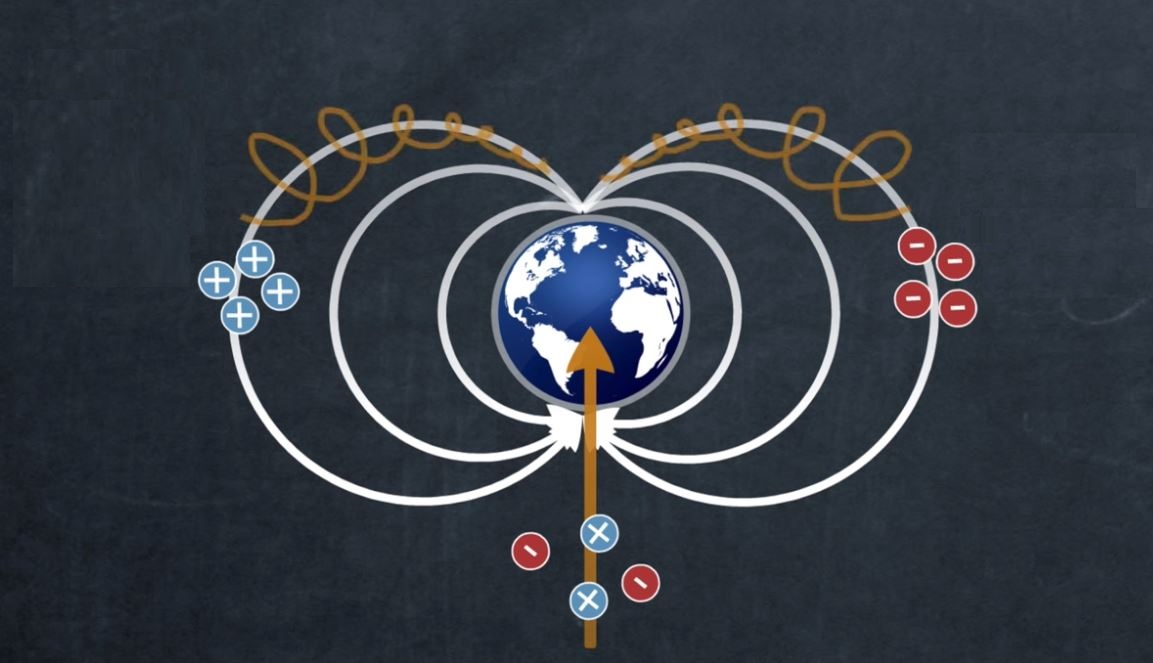
\includegraphics[width=0.9\textwidth]{Elektronenbahnen.jpg}
\end{center}
\end{frame}
\begin{frame}{Inwiefern schützt das Magnetfeld die Erde?}
\textbf{Entstehung eines Polarlichts - Die Atmosphäre leutet}\pause
\begin{itemize}
    \item Bei den Polen sind die Feldlinien senkrecht zur Erdoberfläche. Den Teilchen gelingt es dort in die Atmosphäre einzudringen.\pause
\item Sie treffen auf Sauerstoff- \& Stickstoffatome der Atmösphare.\pause
\item Beim Zusammenstoß werden die Atome angeregt (Elektronen werden auf höhere Energieniveaus gebracht).\pause
\item Die Atome Strahlen daher je nach Höhe in typischen Farben: Sauerstoff Grün, Stickstoff Bläulich/Lila  
%\item Je nach Stärke der Sonnenwinde erscheinen die Lichter in verschiedenen Formen. Nach der Vallance-Jones-Classification können diese zum Beispiel Corona (also ringförmige Strahlen), Vorhänge, Bögen oder Bänder sein.
\end{itemize}
\end{frame}



\begin{frame}{Quellen}
    \begin{itemize}
        \item https://www.planet-schule.de/mm/die-erde/Barrierefrei/pages/Warum\_ist\_die\_Erde\_ueberhaupt\_magnetisch.html
        \item https://de.wikipedia.org/wiki/Erdmagnetfeld
        \item https://www.max-wissen.de/Fachwissen/show/4366
        \item https://www.esa.int/Space\_in\_Member\_States/Germany/Das\_Erdmagnetfeld\_Ein\_riesiger\_Dynamo
        \item https://www.weltderphysik.de/gebiet/erde/erde/erdmagnetfeld/
        \item https://www.welt.de/wissenschaft/article9090079/Was-passiert-wenn-das-Erdmagnetfeld-kollabiert.html
        \item https://praxistipps.focus.de/wie-polarlicht-entsteht-einfach-erklaert\_108114
    \end{itemize}
\end{frame}

\end{document}
